\addchapheadtotoc
\chapter{Security CAT - Proof of Concept Implementation}

This chapter introduces the Proof of Concept setup and architecture of the Security Compliance Automation Tool. It gives an overview of general components and the implemented microservices. 

\section{Architecture}
\label{architecture}
Considering the nature of the testing and evaluation system described in \ref{secCat}, a microservice architecture with loose coupling of the core components, is required. Simple extendability and delegation from SecurityRAT are the focus points in the design.
The architecture incorporates already validated efforts done in \citep{secCat2020}. Parts of the architecture have been adjusted to support lengthy running evaluations and increase the level of abstraction.

The below schematic drawing visualizes the entities and interconnections of SecurityCAT.

\newpage

\begin{figure}[ht!]
\begin{center}
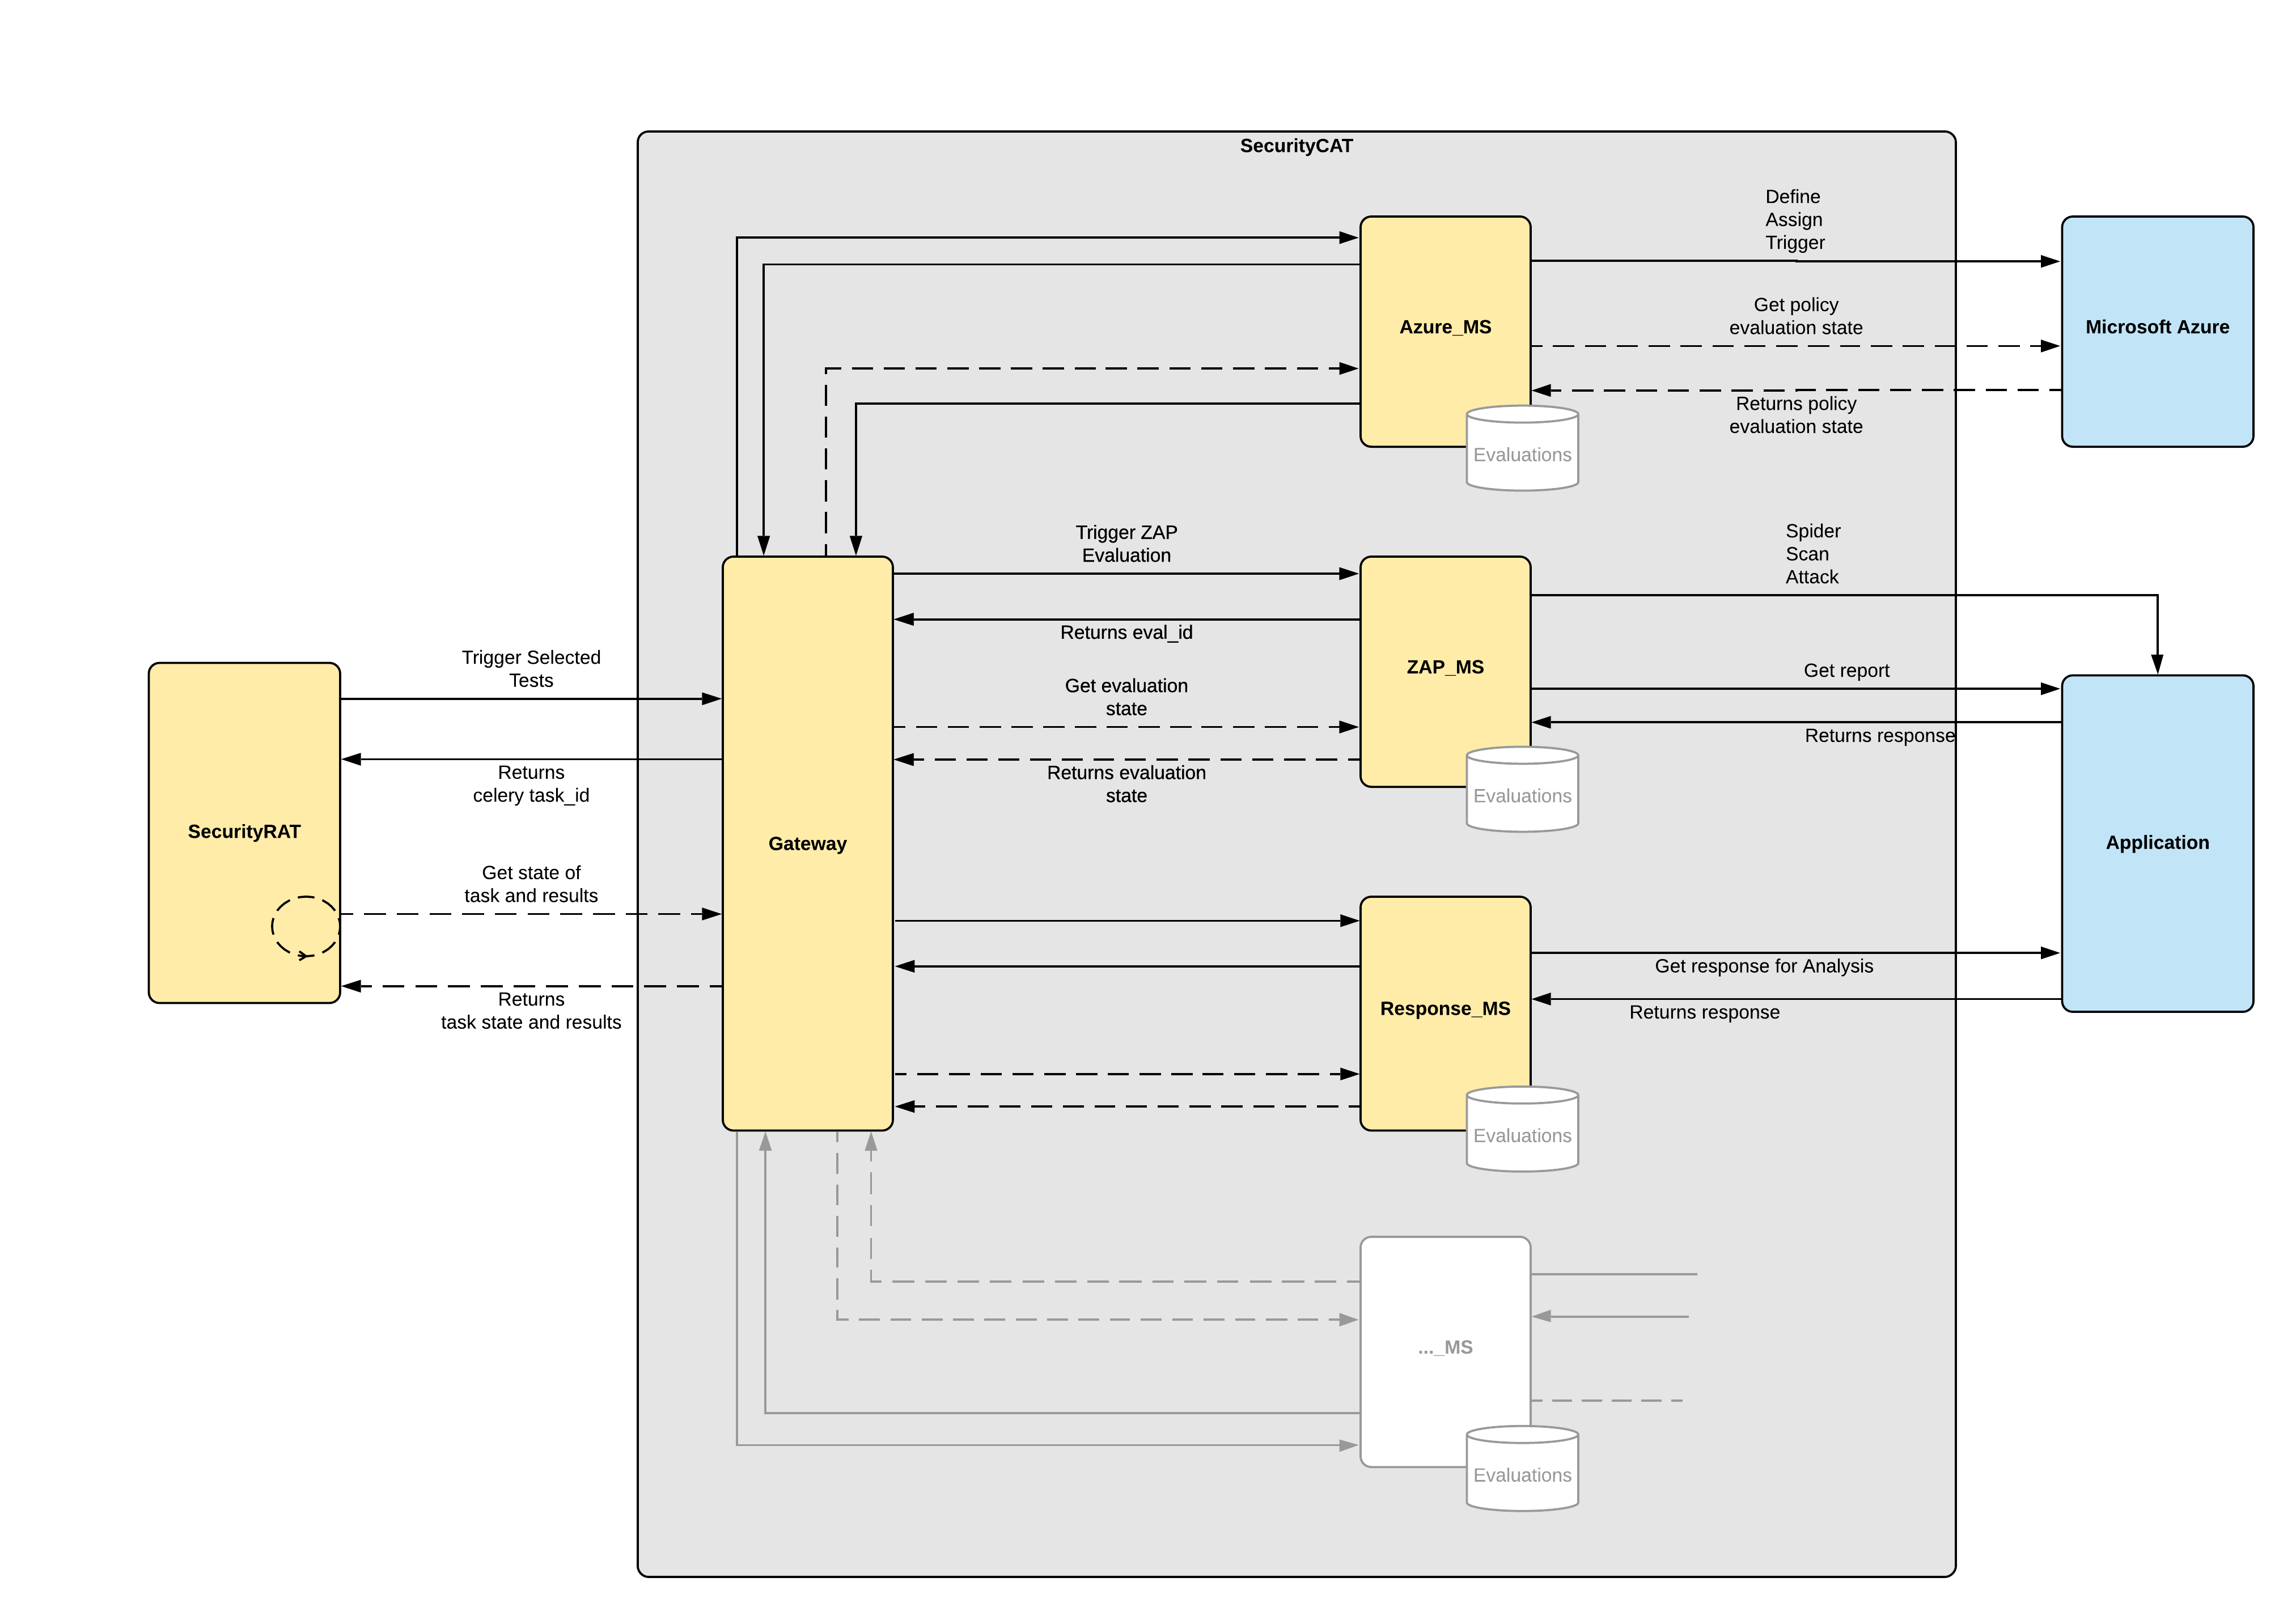
\includegraphics[width=17cm]{SecurityCAT_Architecture.png}
\end{center}
\caption[SecurityCAT architecture]{SecurityCAT architecture}
%Source:
\end{figure}

SecurityRAT serves as a single source of truth for the management of the given project. Only information persisted in SecurityRAT is recognized as acceptable, and any information gathering starts there.

Selecting and testing requirements trigger the process of delegating them to the gateway of SecurityCAT. The gateway further delegates the requirements to the microservices depending on the to be tested properties. SecurityCAT creates a celery task for each test evaluation and returns the according to celery \boldsymbol{task\textunderscore id} to SecurityRAT. This \boldsymbol{task\textunderscore id} is then used to check the progression state and result of the evaluation regularly with a given interval.

Each microservice is passed only the information necessary for the evaluation. Upon triggering the test evaluation, a microservice returns a \boldsymbol{eval\textunderscore id} to the gateway. This \boldsymbol{eval\textunderscore id} is used to check the state of evaluation once SecurityRAT checks in at the gateway for the state of test evaluation.
Each microservice has its additional elements described in their according sections of this thesis. They are not displayed in the architectural overview. Resources that are accessed and used are not part of SecurityCAT and are defined by the properties defined in the SecurityRAT test creation step.

New microservices can be added by following the format given in \ref{extendability}. The system flow allows long-running and time-consuming evaluations. Especially the policy and compliance evaluation of Microsoft Azure can take several minutes depending on the size of the infrastructure.


\section{Automated Infrastructure Testing}
\label{automated_infrastructure_testing}

\subsection{Microsoft Azure Policies}
Not every internal requirement is easily testable with a given Azure policy. Organizational requirements, as stated before, as well as more complex technical requirements like protection against application-level security threats, can not be tested this way.

Upon triggering of the test execution, SecurityRAT sends the information of the selected requirements to the gateway of SecurityCAT. The gateway then delegates the requirement tests, according to their names, to the microservices. Azure specific requirements that have an associated policy are delegated to the Azure microservice. The microservice tests the policies in Azure by triggering configuration checks.

The schematic structure of this setup looks like this.

\newpage

\begin{figure}[ht!]
\begin{center}
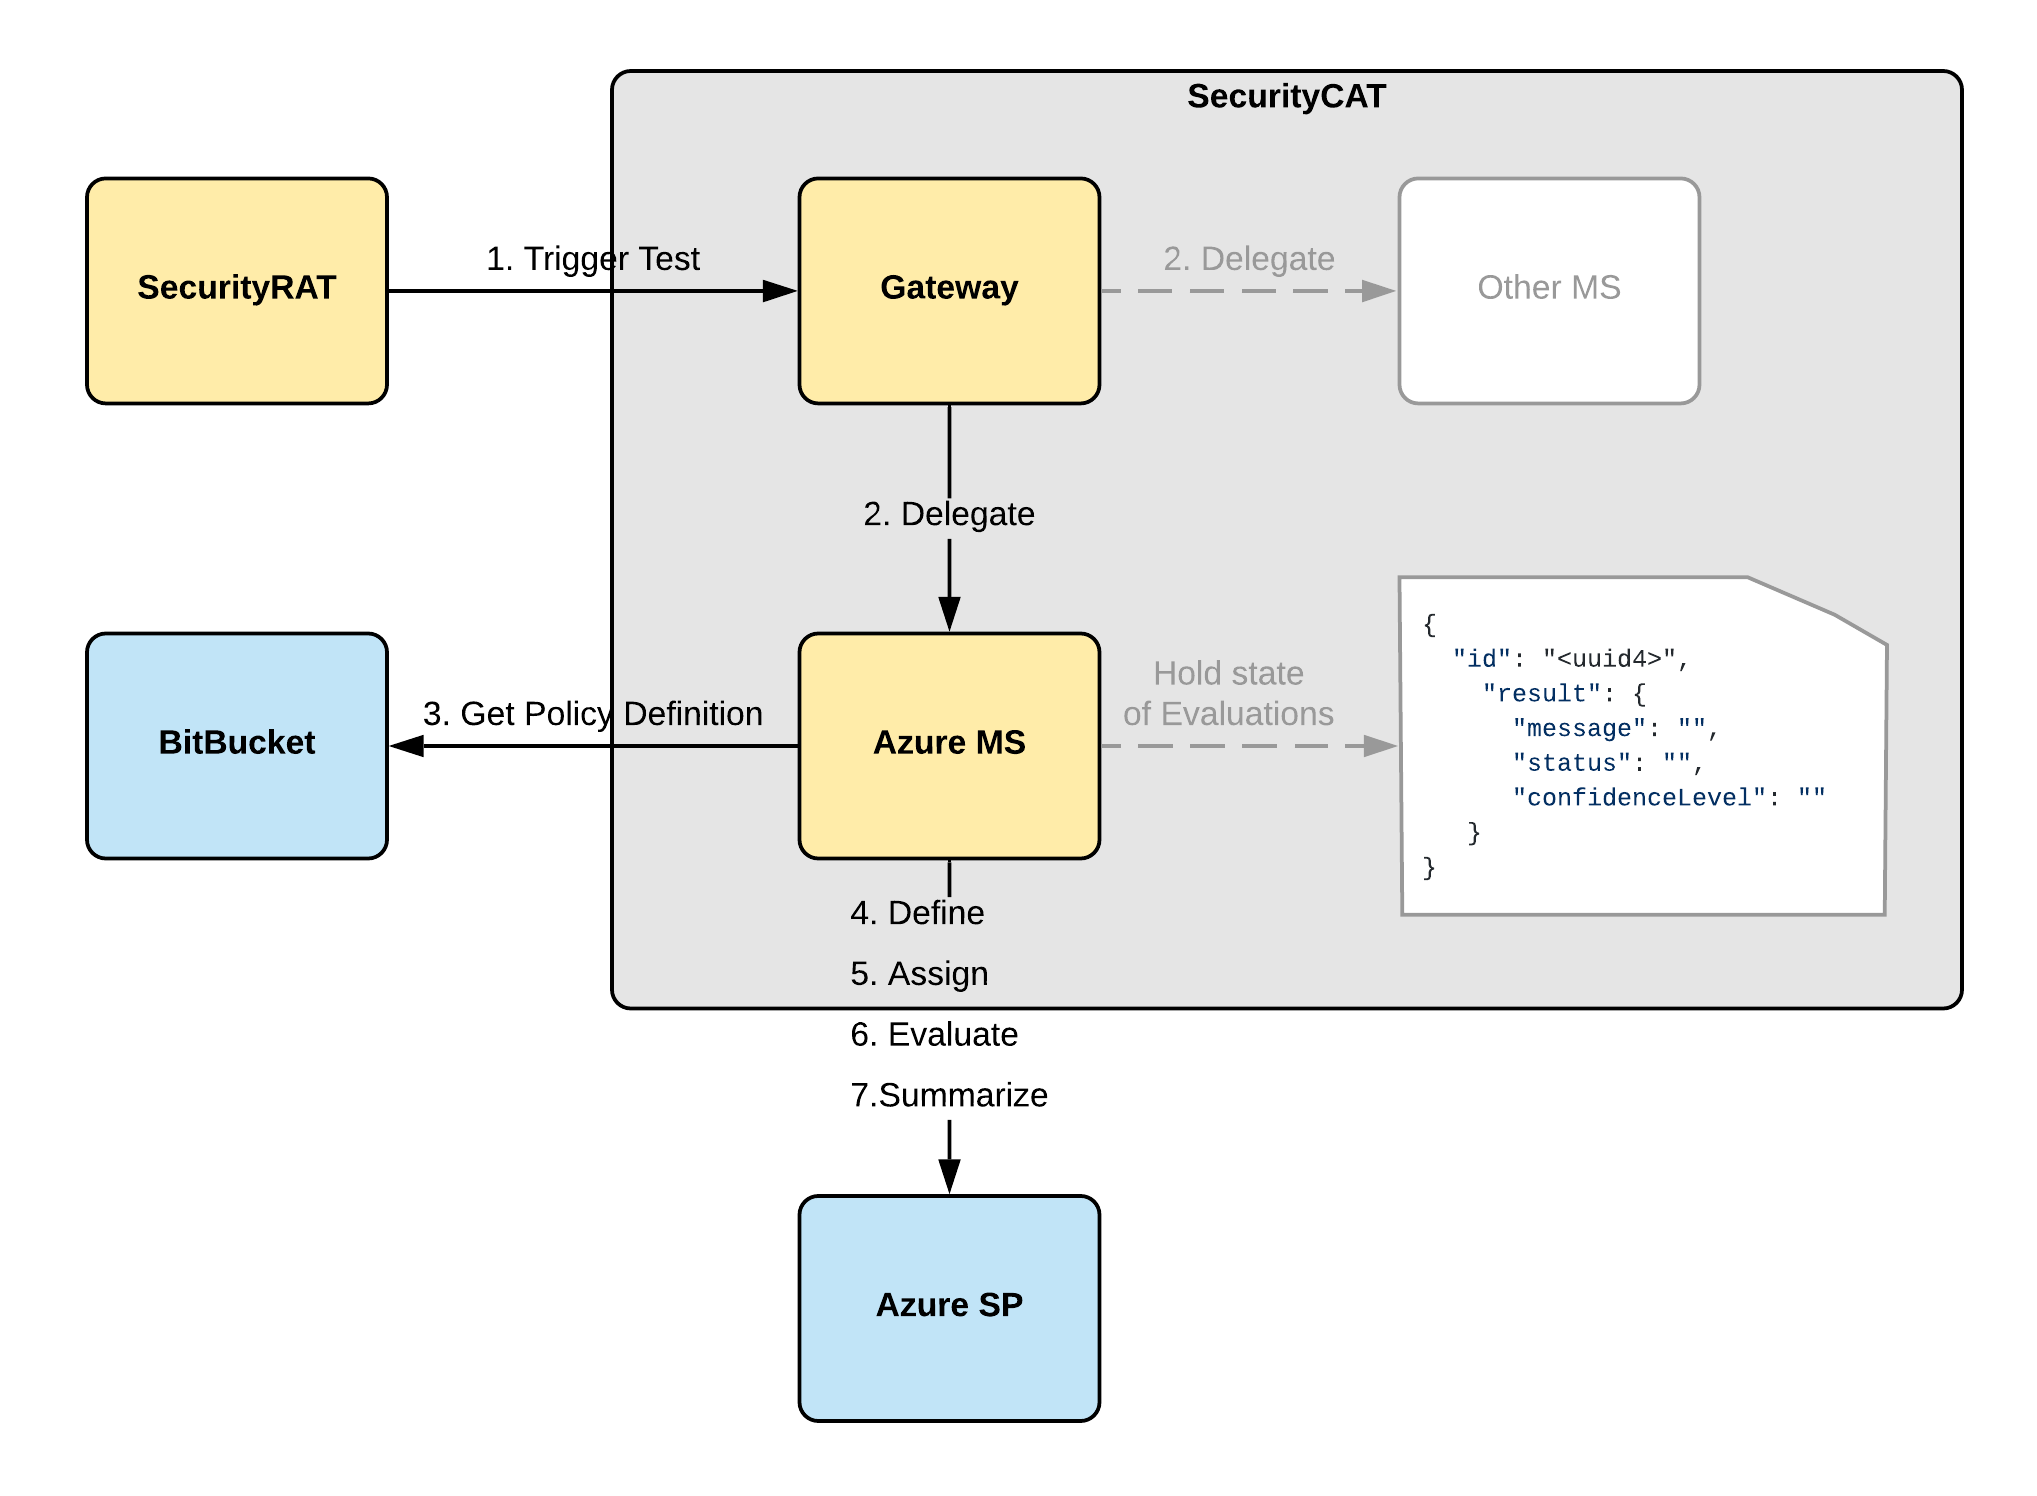
\includegraphics[width=15cm]{Azure_MS_flow.png}
\end{center}
\caption[SecurityRAT to Azure MS schema]{SecRAT to Azure MS schema}
%Source:
\end{figure}

Each Policy Evaluation is handled in a separate thread in the microservice. The policy definitions, assignments, and evaluations are done separately for each requirement.
The current state and final result of each evaluation are persisted in memory for the given evaluation-id. As described in \ref{architecture}, this is one of the critical sections of the architecture at the moment but can be easily replaced with a database in the progression from PoC to implementation. 

The definition, assignment, evaluation, and summarization flow is an essential part of the Azure microservice (Azure MS) since Azure requires a strict execution flow.
The main interaction flow between the microservice and Azure can be described as follows:

\newpage

\begin{figure}[ht!]
\begin{center}
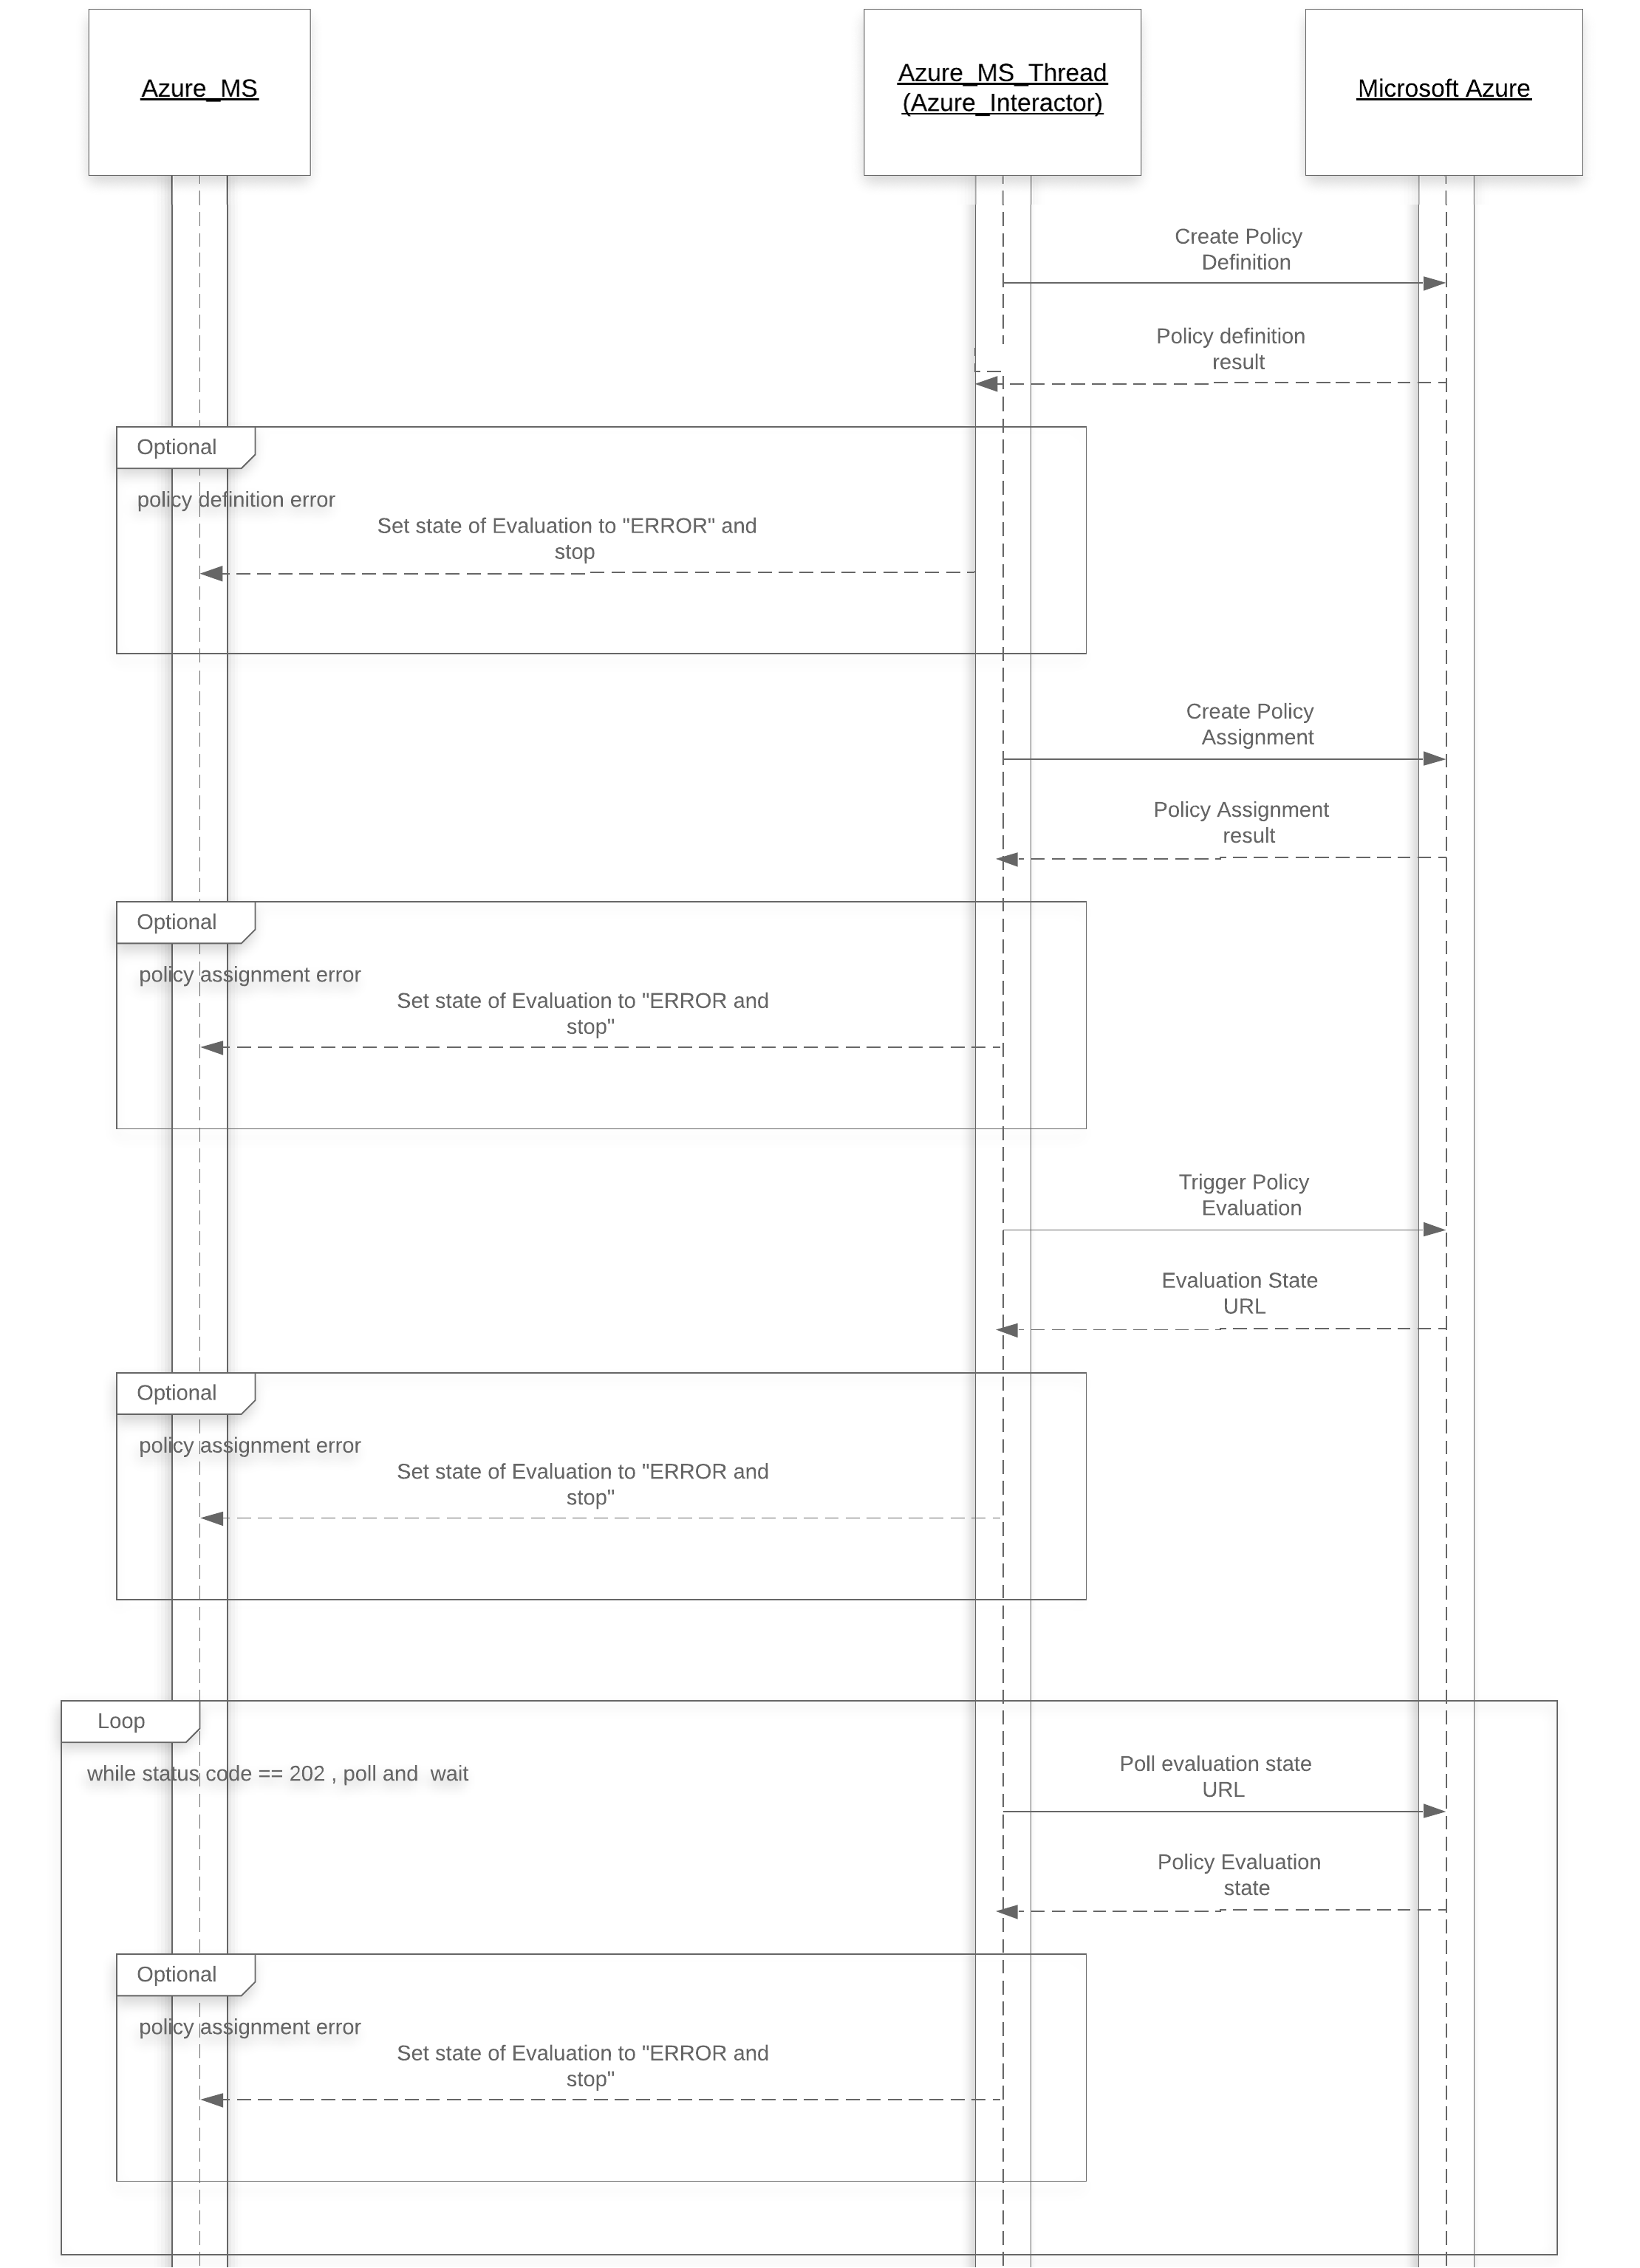
\includegraphics[height=20cm]{Azure_MS_Sequence_cropped.png}
\end{center}
\caption[Azure Policy MS sequence flow]{Azure Policy MS sequence flow. Full chart in Appendix \ref{azure_ms_sequence_chart}}
%Source:
\end{figure}

\vskip 1cm

The central part of the Azure microservice is the policy definitions. They define the expected behavior of a resource and can be tested against specific resources of the target system.

In order to get access to the Azure Policy system, a new application needs to be registered and authenticated using what is called a Service Principal. A service principal is bound to four pieces of information, a \boldsymbol{tenant\textunderscore id} of an Azure subscription, the \boldsymbol{client\textunderscore id} and \boldsymbol{token} (secret) of the registered application, and a \boldsymbol{resource} scope.

After the authentication process, policies can be uploaded, assigned, and triggered. The following example policy definition explains the structure and entities.

\vskip 1cm

\begin{lstlisting}[ backgroundcolor = \color{gainsboro}, 
                    xleftmargin = 2cm, 
                    framexleftmargin = 1em, 
                    language=JSON,
                    caption={Azure Policy Example},
                    captionpos=b]
{
"properties": {
    "displayName": "[MSA-0.0.1] - 
                        Single Contact in Subscription",
    "policyType": "BuiltIn",
    "mode": "Indexed",
    "description": "MSA-0.0.1 - Security contact must 
                                be set for Subscription",
    "metadata": {
      "category": "MSA"
    },
    "policyRule": {
      "if": {
        "field": "type",
        "equals": "Microsoft.Resources/Subscriptions"
      },
      "then": {
        "effect": "auditIfNotExists",
        "details": {
          "type": "Microsoft.Security/securityContacts"
        }
      }
    },
    "parameters": {}
  }
}
\end{lstlisting}

Each policy definition needs a \boldsymbol{displayName} that identifies the policy. The \boldsymbol{policyRule} section describes the targeted resources and expected behavior. In the example policy above, compliance is not achieved if security contact information is not given for Subscriptions.

Since the behavior of the check is defined through a standardized configuration file, the whole process of policy evaluation can be easily abstracted. 


\subsection{Amazon Web Services Config Rules}
\label{awsConfigRules}
Amazon Web Services (AWS) has a comparable system to test the compliance of infrastructure setup. The so-called, Config Rules are serverless Functions (Lambdas) that can be executed to test given resources for their compliance with the expected behavior.
Other than the simple policy definition configuration files on the Azure platform, the Config Rules are small programs written in one of the supported programming languages. This provides more powerful tooling to the user. However, it also increased the complexity of the creation process.

\newpage

Depending on the complexity of the Config Rule, Unit tests need to be added to ensure the correct working of the given script. AWS provides a list of useful config rules, like checking whether the volume encryption for computing resources is enabled. 

\begin{figure}[ht!]
\begin{center}
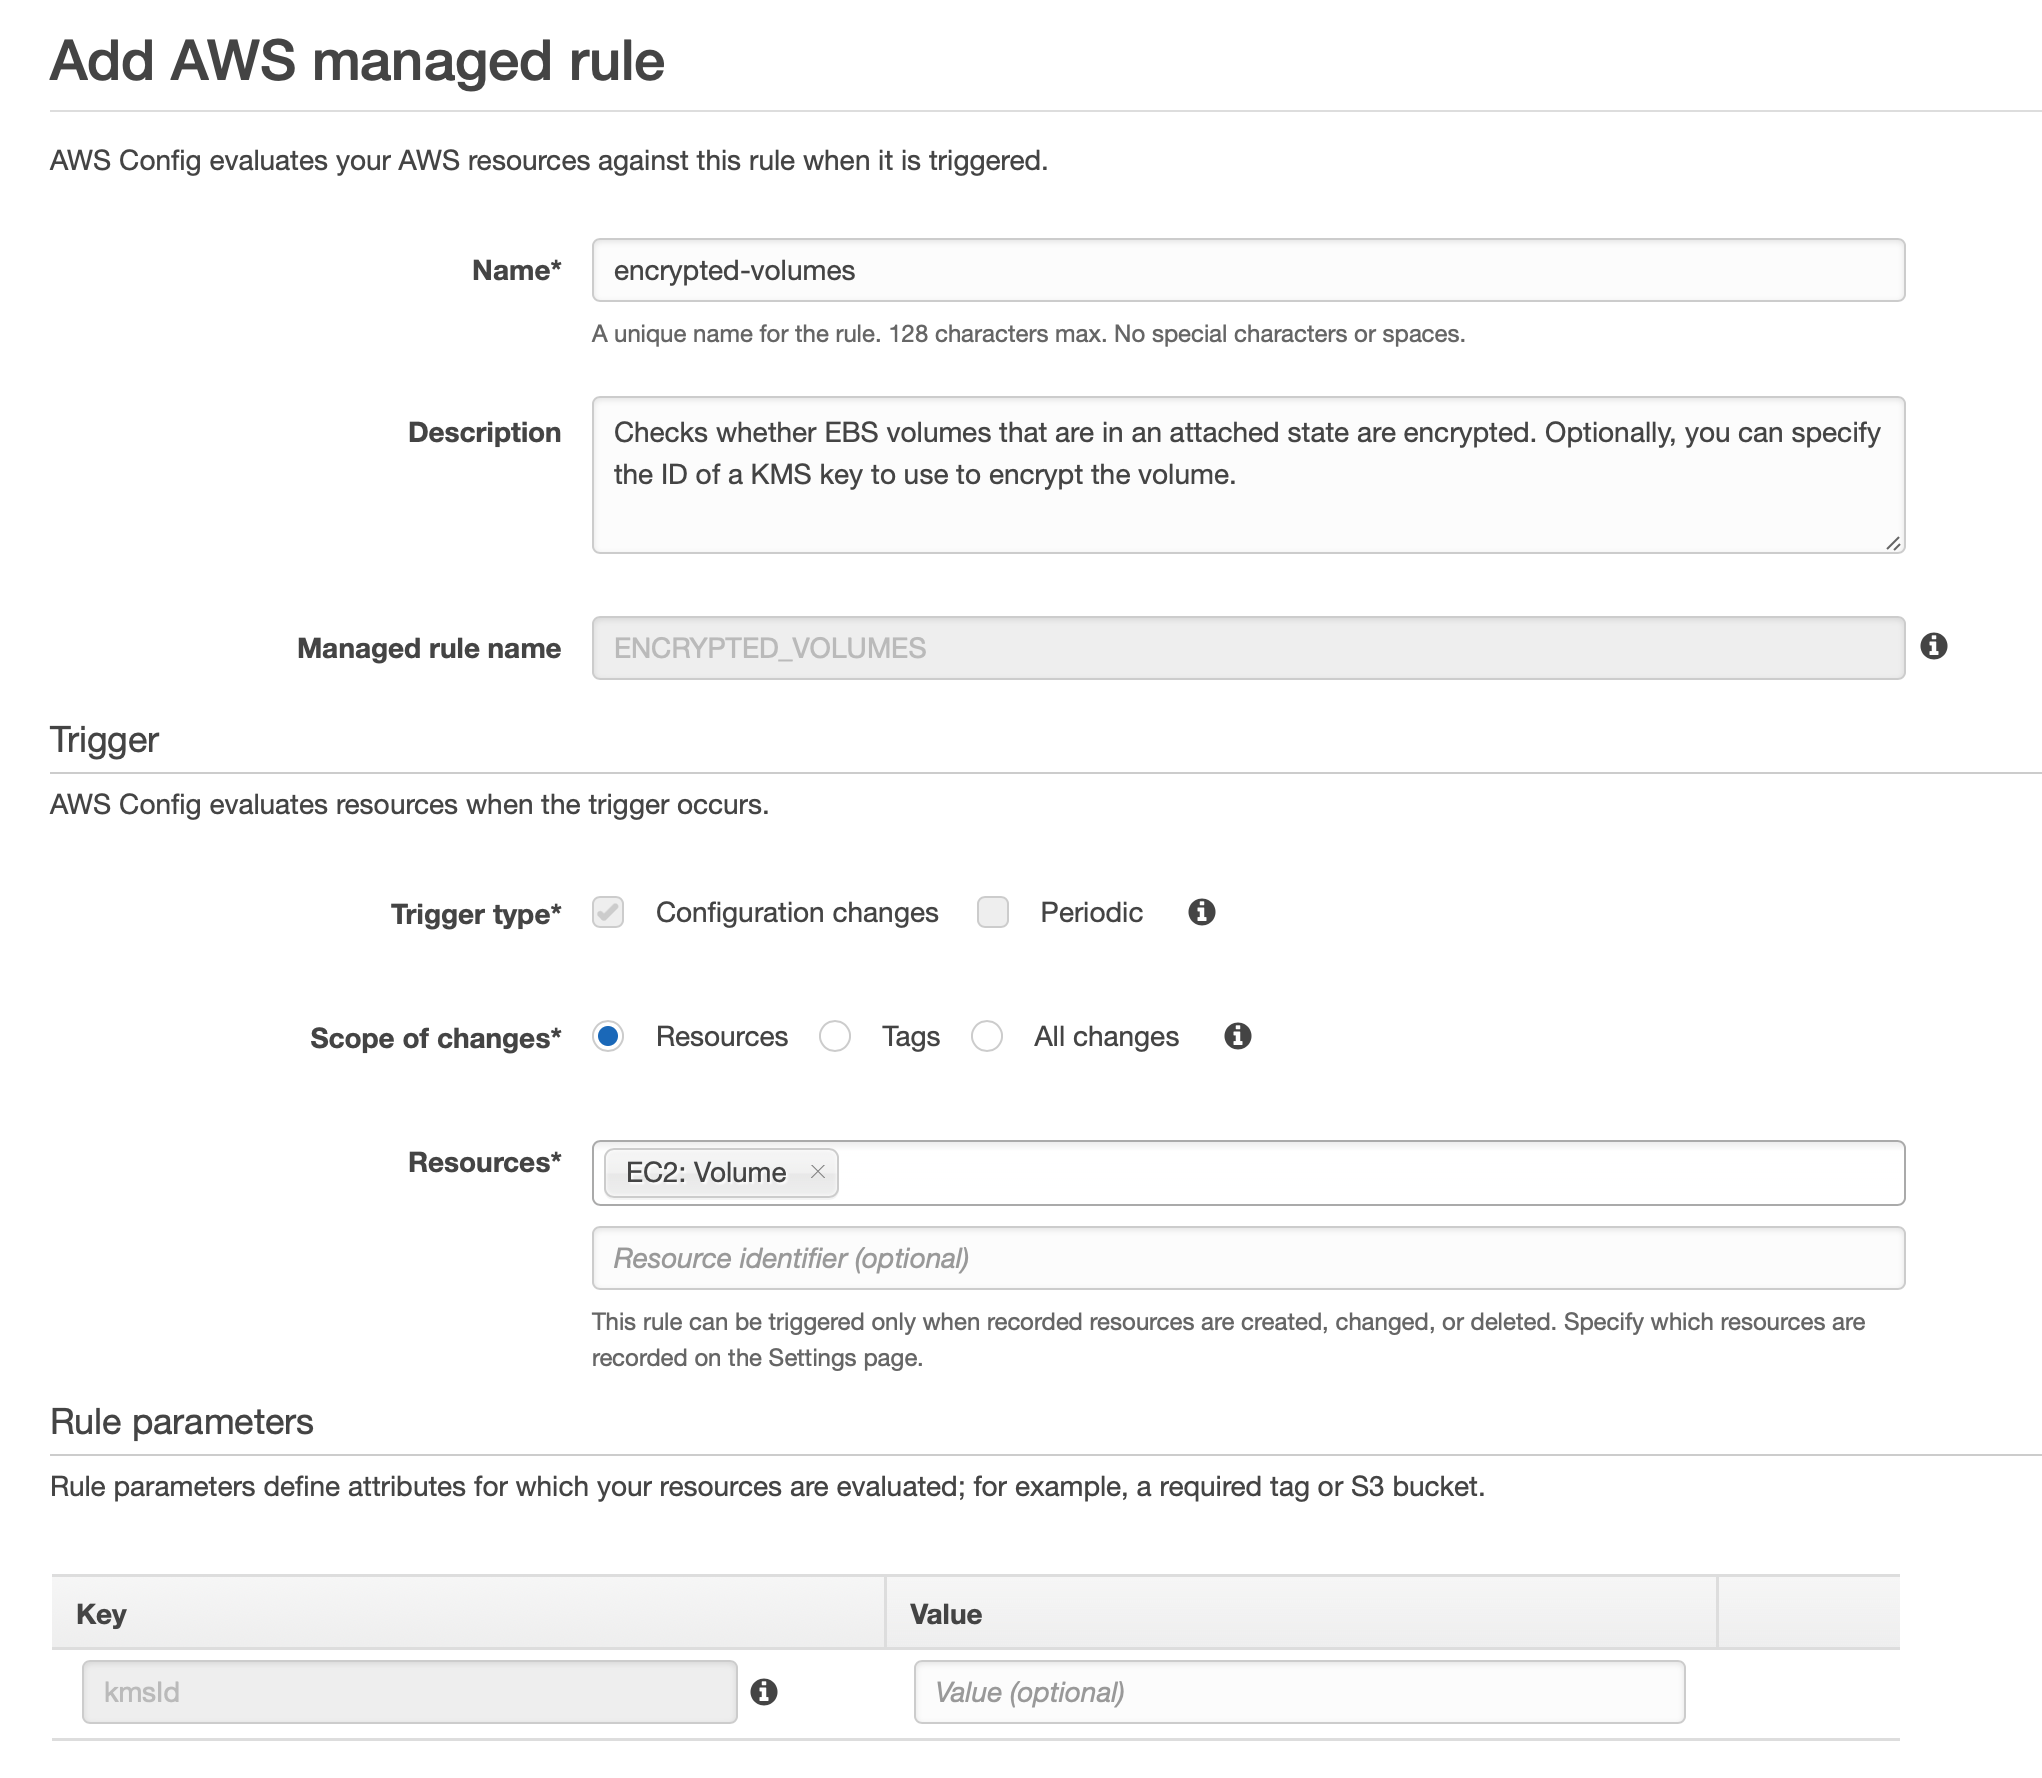
\includegraphics[width=15cm]{aws_config_rule_example.png}
\end{center}
\caption[EC2 Volume Encryption example Config Rule]{EC2 Volume Encryption example Config Rule}
%Source:
\end{figure}

In the AWS console, we can customize the provided config rules and define which resources should be affected and evaluated.
The management of the rules can be automated similarly, like the Azure Policies. A simple authentication flow, followed by describing, activating, and triggering the rule, can be created using the \boldsymbol{boto3} python library.

As part of this thesis, only one platform, Azure, has been covered and implemented.


\section{Automated Application Testing}
\subsection{Security Testing ZAP}
\label{zapTesting}
In contrast to infrastructure testing, applications have no strict underlying configuration that can be easily tested for misconfiguration using something like polices.
As briefly introduces in \ref{autoPentTesting}, the ZAP Proxy will serve as the automated security testing assessment tool for the PoC implementation.
The problems described in the conceptual chapter already introduced the existence of problems such as low confidence levels for problems and the vast amount of potential false negatives. When compared to automated infrastructure testing, we can not merely fully trust the results of the automated test but have to double-check manually.

\begin{figure}[ht!]
\begin{center}
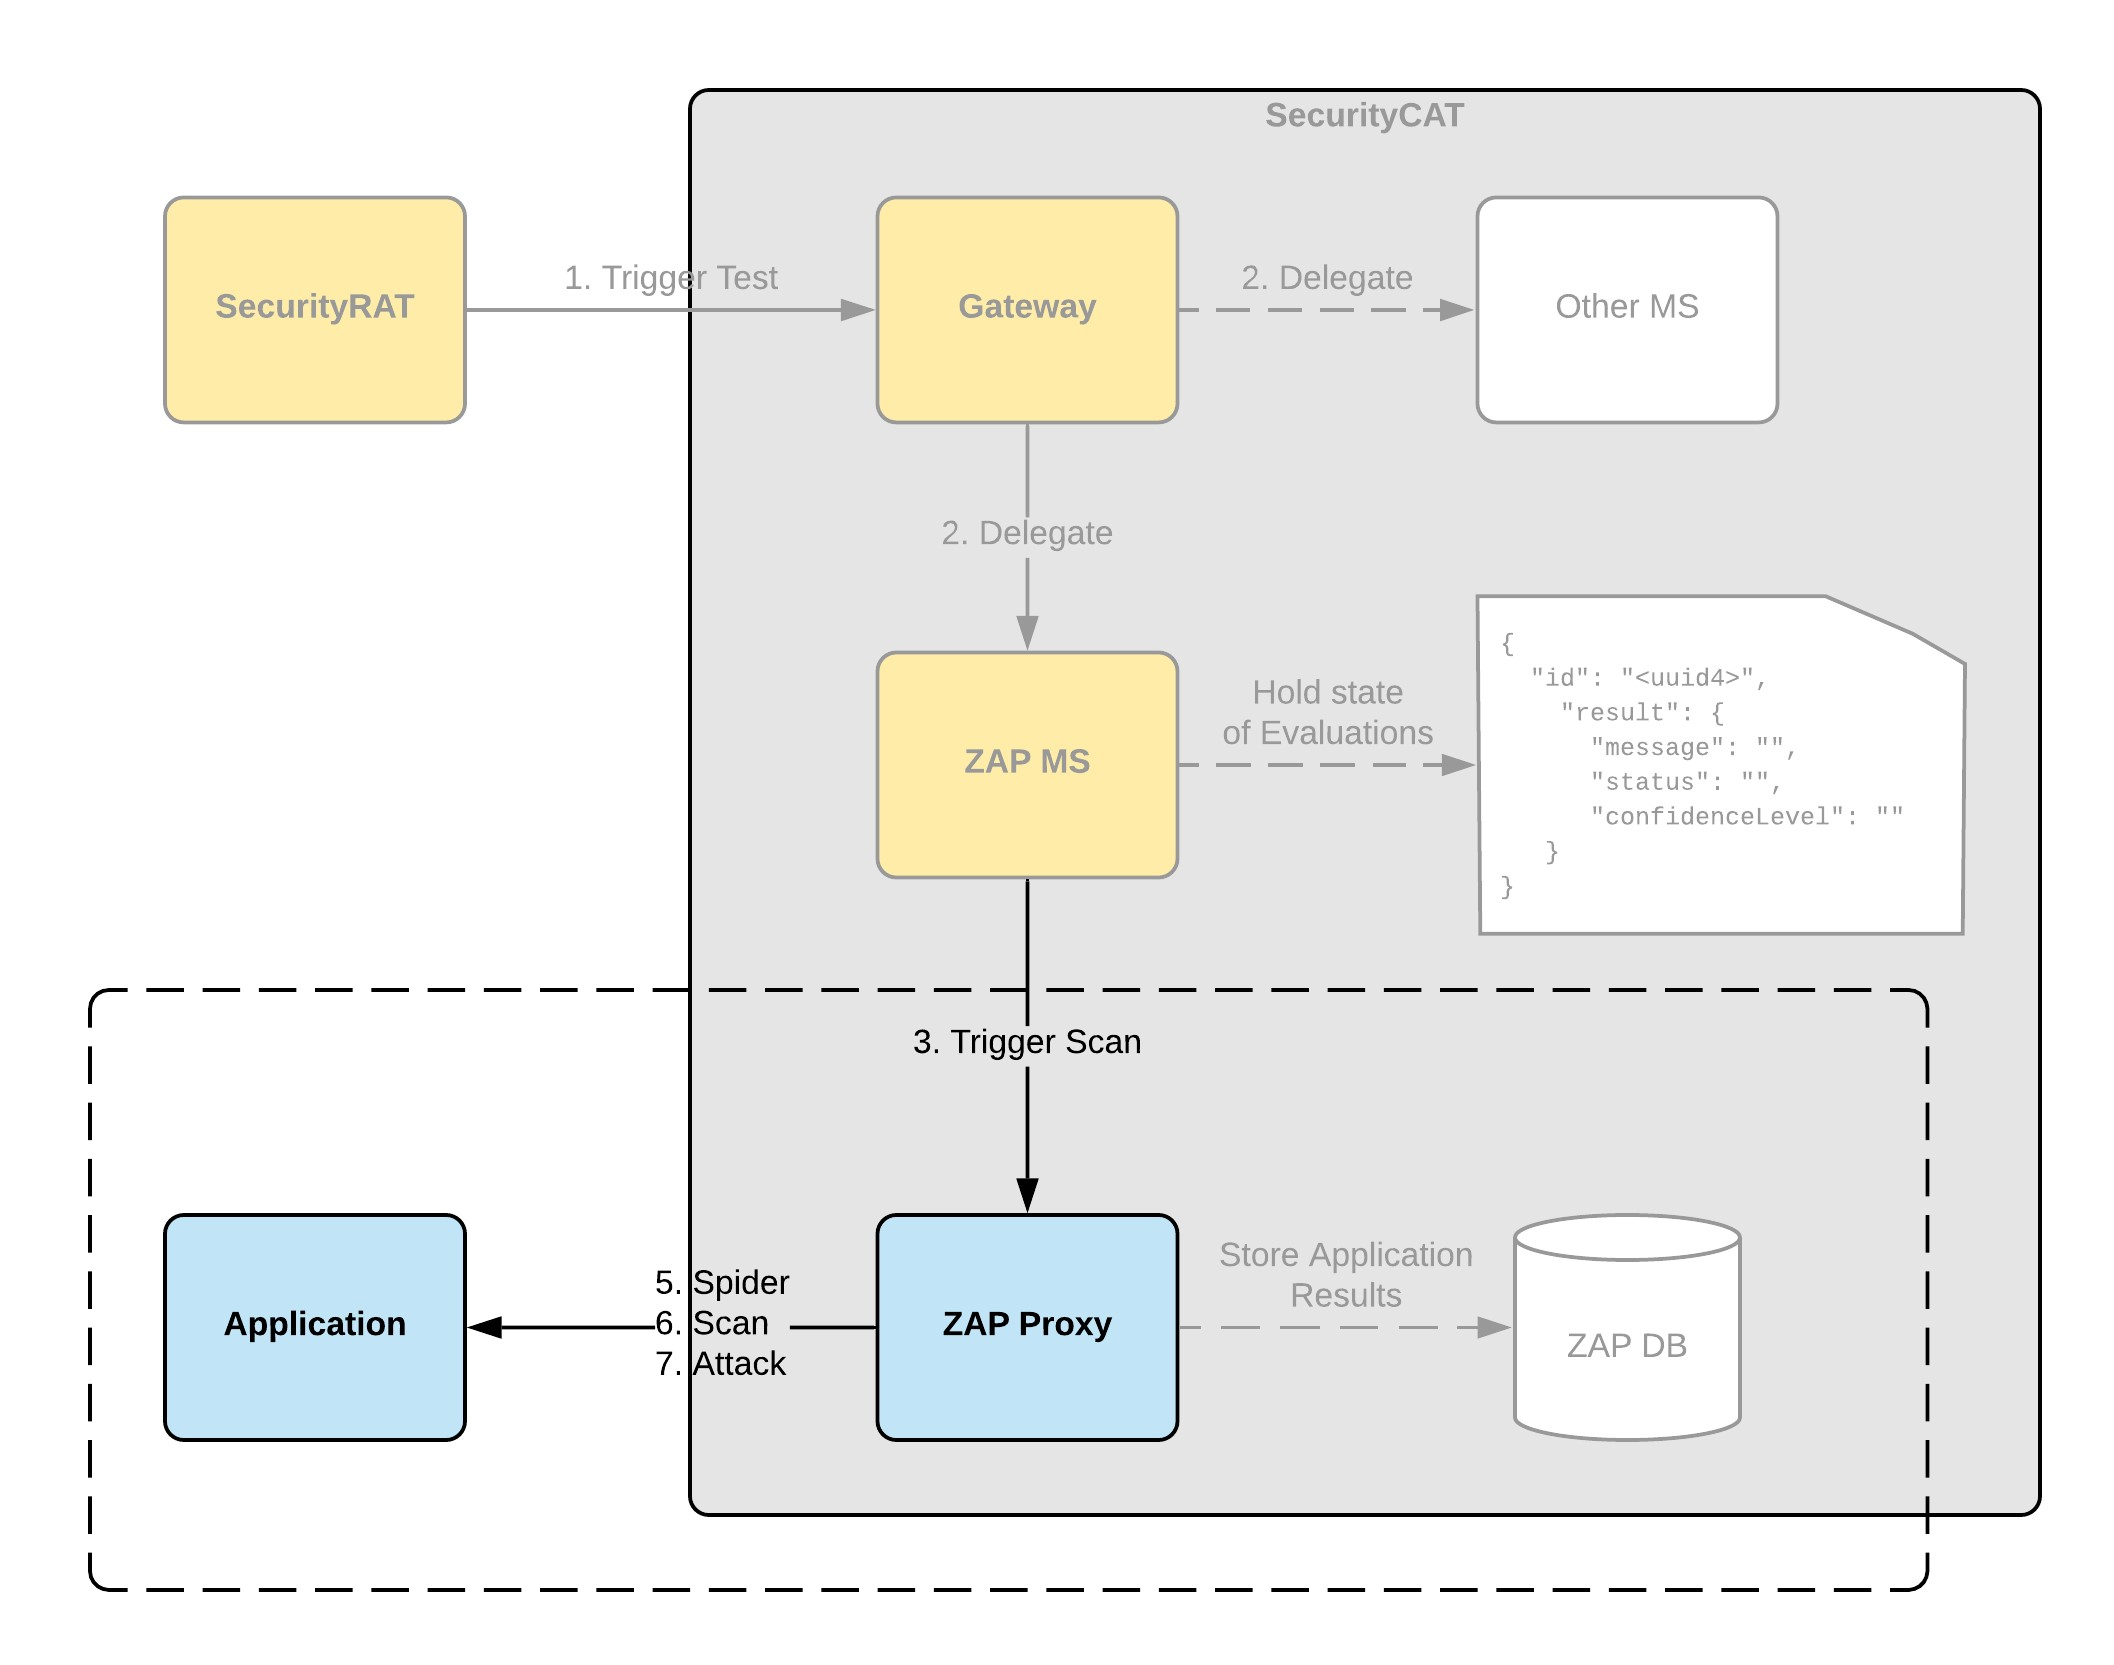
\includegraphics[width=15cm]{ZAP_MS_flow.jpg}
\end{center}
\caption[ZAP microservice flow with highlighted ZAP specific section]{ZAP microservice flow with highlighted ZAP specific section}
%Source:
\end{figure}

The schematic drawing shows the generally described format of the microservices and highlights the ZAP specific section of it. The microservice triggers the execution of a series of steps on a ZAP session. ZAP spiders, scans, and attacks the provided application and persists all found vulnerabilities and faulty configurations in its accompanying database. Once the full attack flow has been performed, the microservice gets the final report from the ZAP Proxy and provides the evaluation result for the querying of the gateway.

One problem with this approach is that ZAP only gives precise feedback. It can, for example, detect the presence of possibly security-critical information, exposed in the cookie header of a request. This information, however, has no direct mapping to one of the internal requirements that are listed in SecurityRAT.

The generated JSON report, therefore, has to get an additional mapping step, which helps categorize the found vulnerabilities and errors according to the internal requirements.
The structure of a found alert looks like this.

\vskip 1cm

\begin{lstlisting}[ backgroundcolor = \color{gainsboro}, 
                    xleftmargin = 2cm, 
                    framexleftmargin = 1em, 
                    language=JSON,
                    caption={ZAP Proxy \enquote{Header Not Set} Example Report},
                    captionpos=b]
{
   "alert":"X-Frame-Options Header Not Set",
   "riskcode":"2",
   "confidence":"2",
   "riskdesc":"Medium (Medium)",
   "desc":"<p>X-Frame-Options header is not included
          in the HTTP response to protect against
          'ClickJacking' attacks.<\/p>",
   "instances":[
      {
         "uri":"https://...",
         "method":"GET",
         "param":"X-Frame-Options"
      },
      .
      .
      .
   ],
   "count":"60",
   "solution":"<p>Most modern Web browsers...<\/p>",
   "reference":"<p>http://blogs.msdn.com/...<\/p>"
}
\end{lstlisting}

Each alert has some additional fields. Those fields, however, are not of value for now. The most critical pieces of information are the alert itself, its confidence, the riskdesc (severity), and the description. This information can be used to determine whether a requirement has failed or succeeded.

As mentioned above, since those results are dynamic and follow no strict model, they have to be manually checked for false positives. They can not be used as a final proof for a defined level of security.


\subsection{Custom Response Testing Script}
\label{customTestingScript} 
Standards like ASVS \citep{asvs4.0}, described in \ref{asvsStandard}, and an RFC of the HTTP/s protocol \citep{httpRFC} itself describe several security considerations when it comes to information transfer using HTTP/S.

Many of the given requirements specifically target the header values of an HTTP response. An example for this is the \enquote{ASVS\textunderscore 3.0.1\textunderscore 10.11} requirement which states the following:

\newpage

\begin{quote}
"Verify that HTTP Strict Transport Security headers are included on all requests and for all subdomains, such as Strict-Transport-Security: max-age=15724800; includeSubdomains"
\end{quote}

\vskip 1cm

Since HTTP headers are standardized, checking for their existence and value conformity can be automated. The response check microservice is aimed at not only testing the existence and value of headers for according to requirements but also provide an evaluation about the existence of non-compliant usage of weak encryption, encodings, and leaked session information. 

The following schema shows the response check microservice specific elements. The more specific "Requirement - Eval Function Mapping" entity is described in more detail in the next paragraph.

\begin{figure}[ht!]
\begin{center}
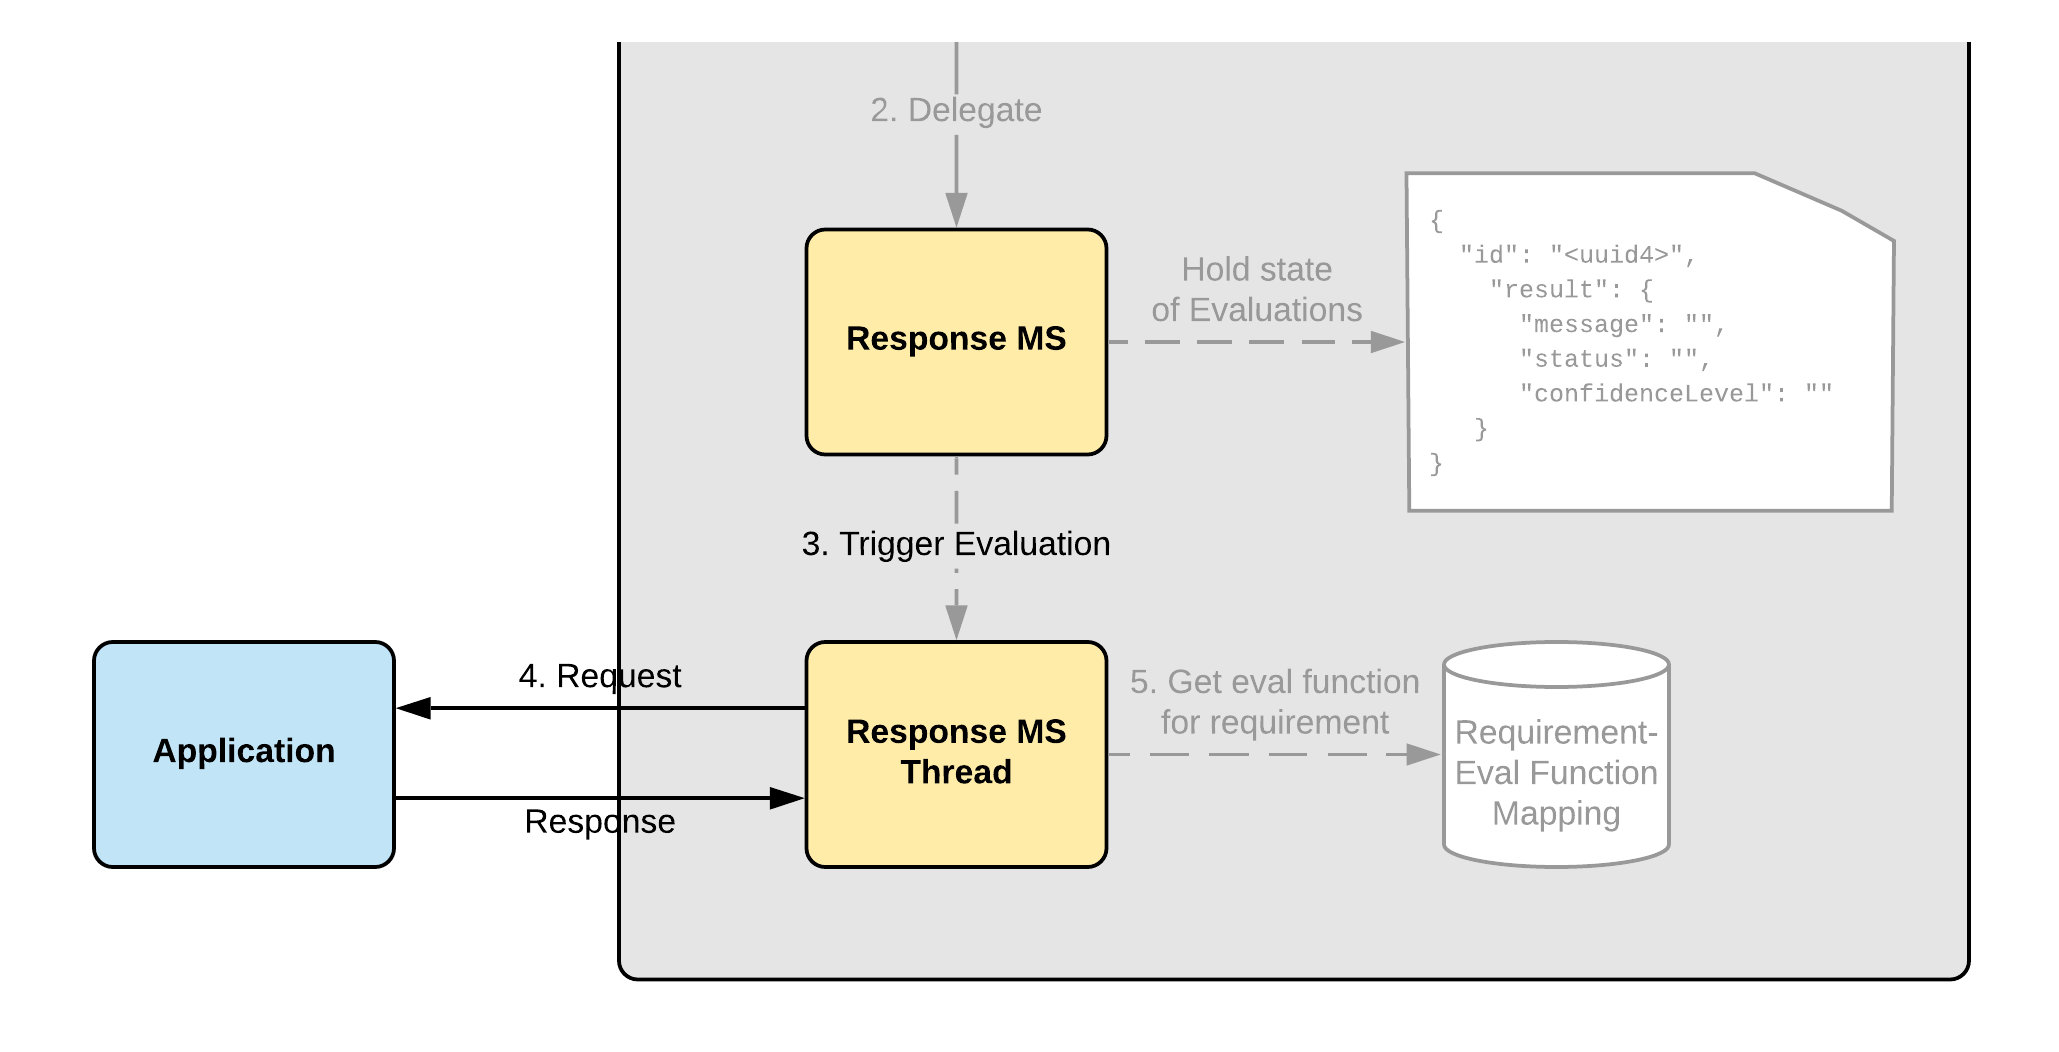
\includegraphics[width=17cm]{Response_Check_MS_flow.png}
\end{center}
\caption[Schematic flow of Response Check Microservice]{Schematic flow of Response Check Microservice}
%Source:
\end{figure}

\newpage

The approach taken for the response check microservice is focused on abstraction and dynamic extendability.
As displayed in the schema above, the basic structure of delegating the evaluation to a worker thread is consistent with all the other microservices.
One of the ways to achieve this abstraction is the introduction of a mapping entity. In a production environment, this can be a database; for this PoC, it is a simple in-memory dictionary. 
Each requirement is mapped to a function, which removes abstraction and provides specific instructions as soon as they become relevant for the evaluation. By using this structure, the implementation can be more general, which results in cleaner, more maintainable code. Requirements and functions can be added or removed at any stage.

The following code snippet displays an example mapping of three ASVS requirements to, so-called, lambda functions in Python.

\begin{lstlisting}[ backgroundcolor = \color{gainsboro}, 
                    xleftmargin = 2cm, 
                    framexleftmargin = 1em, 
                    language=Python,
                    caption={ASVS Requirements to Function mapping},
                    captionpos=b]
__requirement_func_mapping = {
  "ASVS_3.0.1_10.10": lambda headers: 
      __check_headers_contains_elem(
        headers, "Public-Key-Pins"
      ),
  "ASVS_3.0.1_10.11": lambda headers: 
      __check_headers_contains_elem(
        headers, "Strict-Transport-Security"
      ),
  "ASVS_3.0.1_10.12": lambda headers: 
      __check_headers_contains_elem(
        headers, "Strict-Transport-Security", "preload"
      ),
}
\end{lstlisting}

Over time, this microservice should be enriched with a more sophisticated analysis of the HTTP response of the client application. Possible checks include the usage of insecure encodings, exposed session information, guessable session ids, and other, previously mentioned, security considerations.
An important aspect also is the mapping of functionality to the internal requirements maintained by the team. Since those requirements are more general than ASVS, the second step of mapping might need to be introduced upon further experimentation.


\section{Extendability}
\label{extendability}
Considering the architecture described in \ref{architecture}, adding new microservices and extending the system is a streamlined process. As more requirements can be tested, additional microservices can be implemented to evaluate them. Each microservice needs to implement the informal interface in order to keep the communication to the gateway consistent.

Since Python has no concrete concept of interfaces, the approach used here is a very informal one. Documentation and examples should provide a guideline on how new microservices have to be implemented. Once the PoC surpasses the stage feasibility checking, a formal interface based on the used guidelines shall be implemented with the Python-specific tooling.

Each microservice exposes a GET and a POST REST endpoint. A new evaluation is triggered by posting the definition to the POST endpoint. In the example of the Azure policy microservice, this definition is the \boldsymbol{PolicyEvalDefinition} shown in the figure above. This POST call starts a new evaluation and returns the associated \boldsymbol{eval\textunderscore id} to the gateway.
By using the GET endpoint with the given \boldsymbol{test\textunderscore id}, the current state of evaluation and the result, once the evaluation has finished, can be retrieved.

\begin{figure}[ht!]
\begin{center}
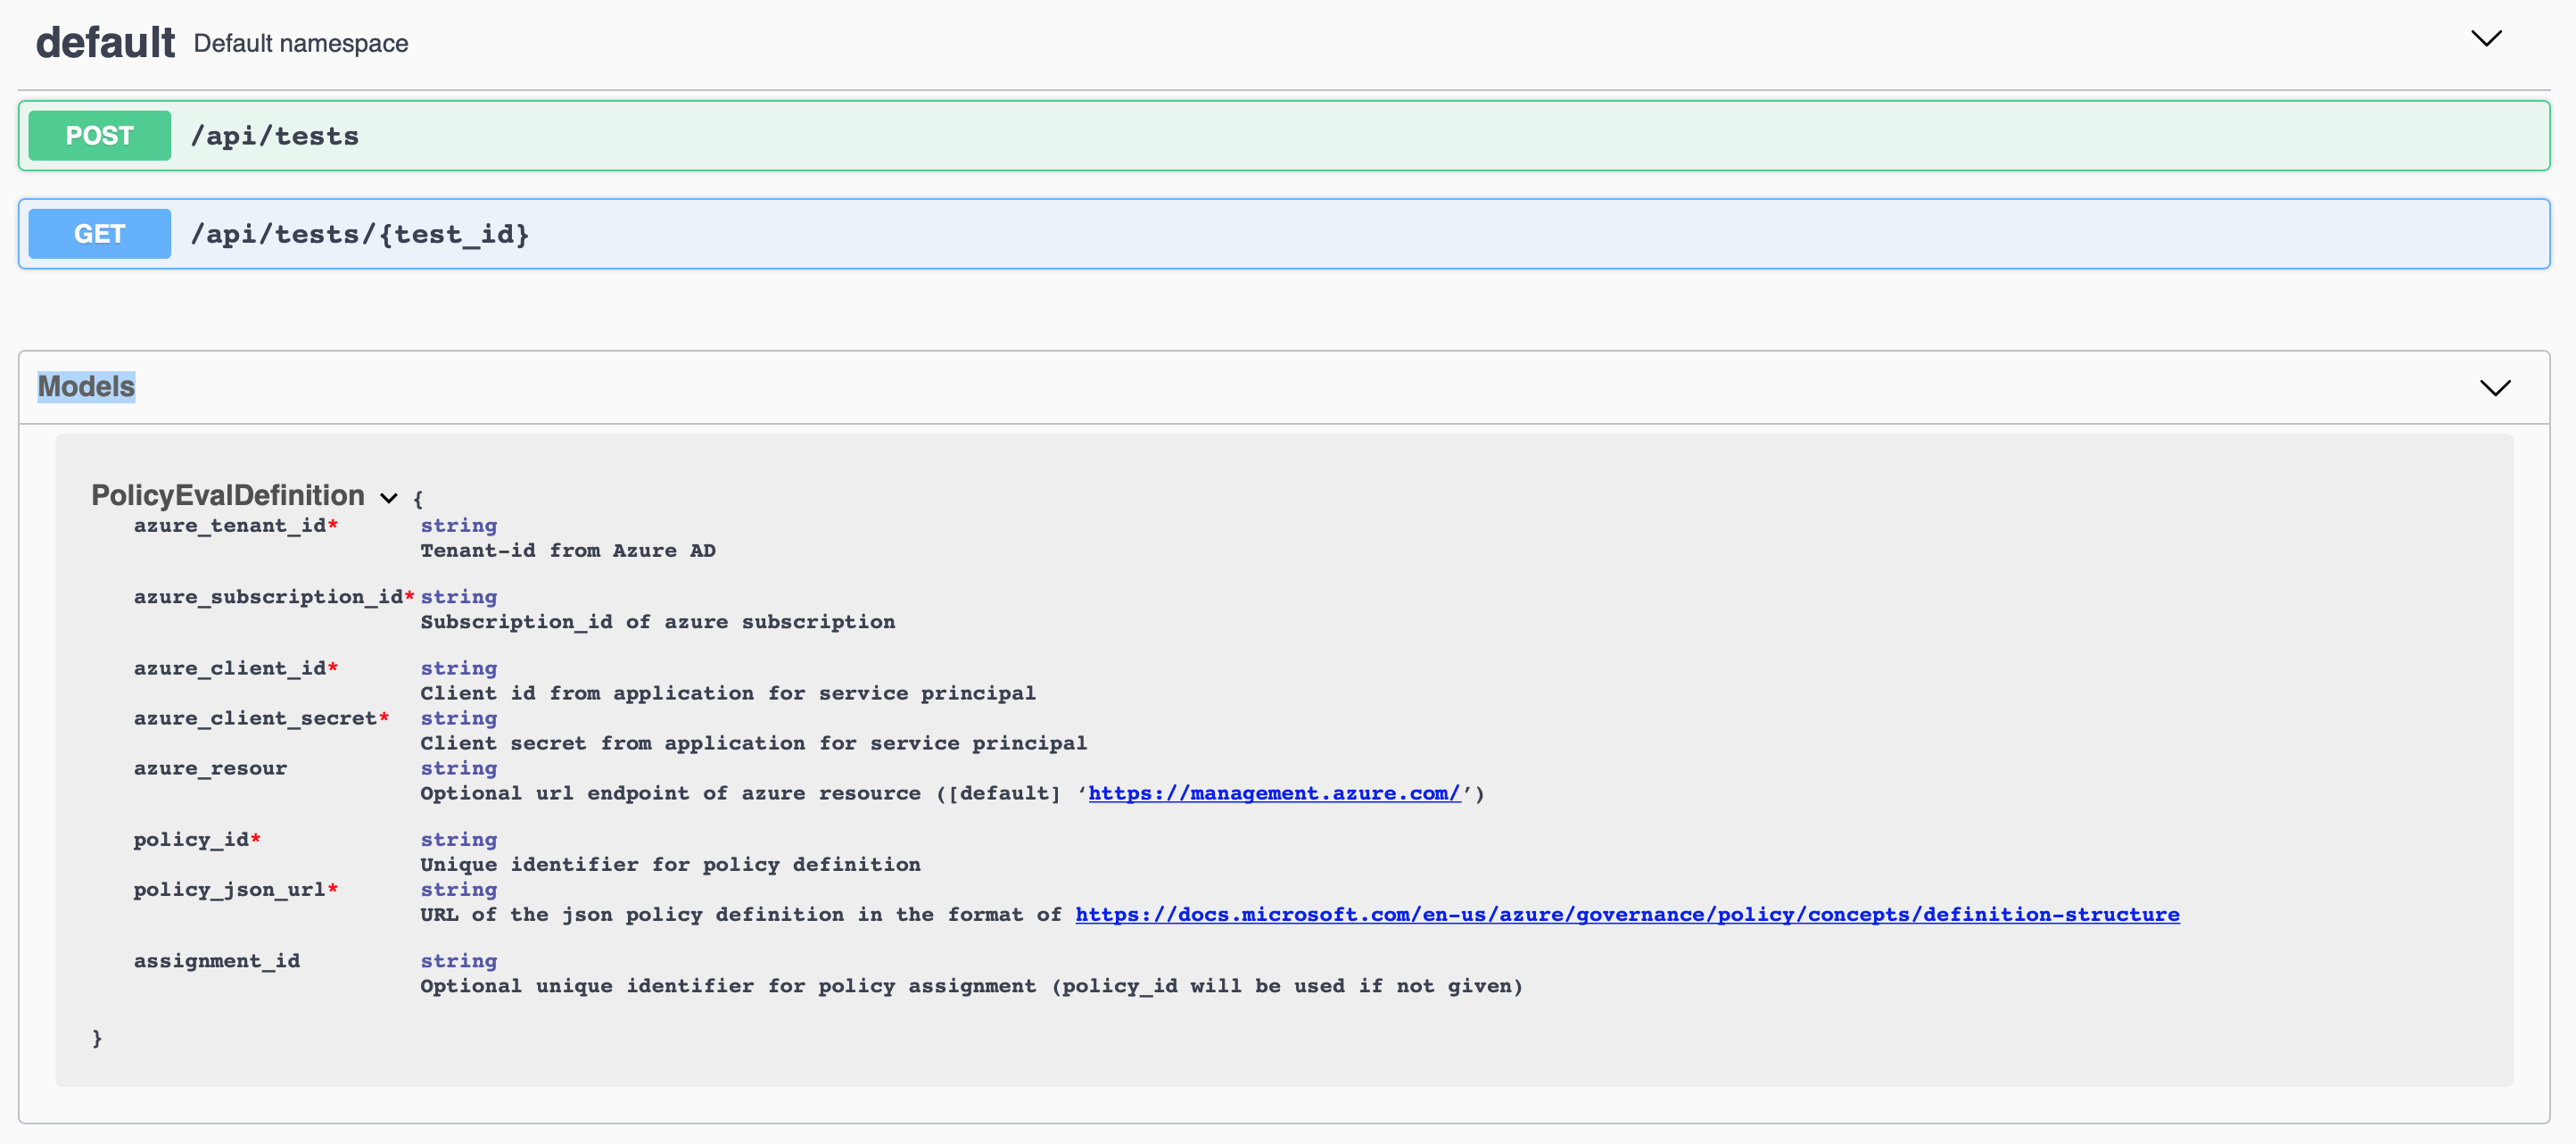
\includegraphics[width=17cm]{swagger_api_azure.png}
\end{center}
\caption[Swagger API documentation of the Azure microservice]{Swagger API documentation of the Azure microservice}
%Source:
\end{figure}